\chapter{Axion analysis}
\label{ch:nedm-at-psi-apparatus}

Now that the foundation of the analysis has been explained we proceed to present how were they applied to the data. The data have been taken at PSI between \ldots during nEDM runs (as in no dedicated runs have been done.)

\mnote{When exactly have the data been taken?}

Explain why short and long time-base analyses. Mention the axion wind analysis already.

In this analysis two couplings were considered. The first  is scalar and looks like an oscillating nEDM. The second is vector and acts like an oscillating magnetic field.

The analysis has been divided in two based also on an another criterium. The long time--base and short time--base. The first used the dataset of the nEDM experiment performed in ILL by the Sussex--RAL--ILL collaboration and covers oscillation periods up to days. The short time--base analysis used the PSI dataset. The latter is the subject of this work, the former is part of the doctoral thesis of Nicholas Ayres \mnote{Cite Nick's PhD here}. We have closely collaborated.



\section{How a signal would look like}
It is instructive to first understand well how would an axion signal come up in the data.

The main purpose of the experiment is to measure the constant neutron electric dipole moment. This would appear as a shift in $R$\mnote{Needs to be clear that the reader is familiar with $R$ here.} dependent on direction of the electric field relative to the magnetic one. In zero electric there would be no shift, while the parallel and anti--parallel configurations of the magnetic and electric fields would shift $R$ in opposite directions. Due to the data blinding
\footnote{In order to reduce bias the data were modified upon being taken in a way, that a secret nEDM was injected into them. This additional offset is only revealed as the very last step, once the measurement and analysis have been completed. The data were still blinded at the time of writing.}
we expect a pronounce shif corresponding to an nEDM $\unit[10^{-25}]{e \cdot cm}$ large.

Should the neutron electric dipole moment oscillate, $R$ would oscillate as well, even if the electric field is kept constant. A reversal of the electric field polarity would reverse the phase of the oscillations. At zero electric field no oscillations would be visible. In Fig.\,\ref{fig:axions_data_taking_one_run} we depict an $R$ time--series with the combined effect of a large nEDM oscillation and the blinding offset.

\begin{figure}[bth]
  \myfloatalign
  \subfloat
  [An oscillating neutron electric dipole moment signal in the nEDM @ PSI apparatus. The colours indicate different electric field states: parallel to the magnetic field, antiparallel to it and zero]
  {\label{fig:axions_data_taking_one_run}
  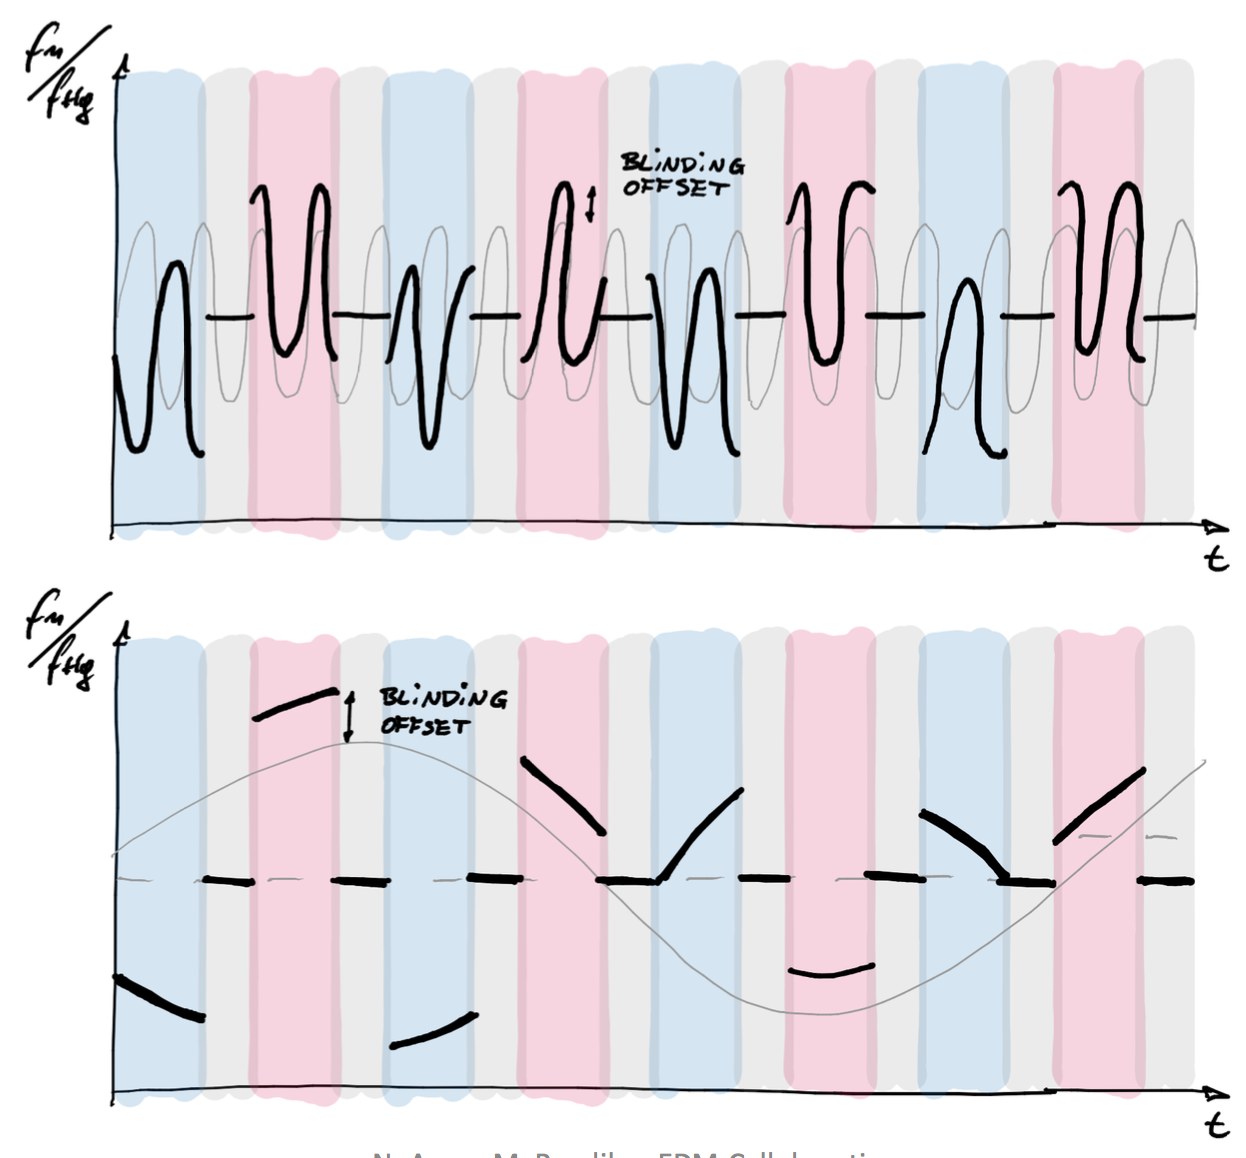
\includegraphics[width=.34\linewidth]{gfx/axions/cycle-level_blinding_offset.png}}
  \quad
  \subfloat
  [An oscillating neutron electric dipole moment signal in the nEDM @ PSI apparatus across many runs. The colours indicate different electric field states: parallel to the magnetic field, antiparallel to it and zero. Different runs have different magnetic field gradients, which causes each run to have a different shift in $R = f_n / f_{Hg}$.]
  {\label{fig:axions_data_taking_runs}
  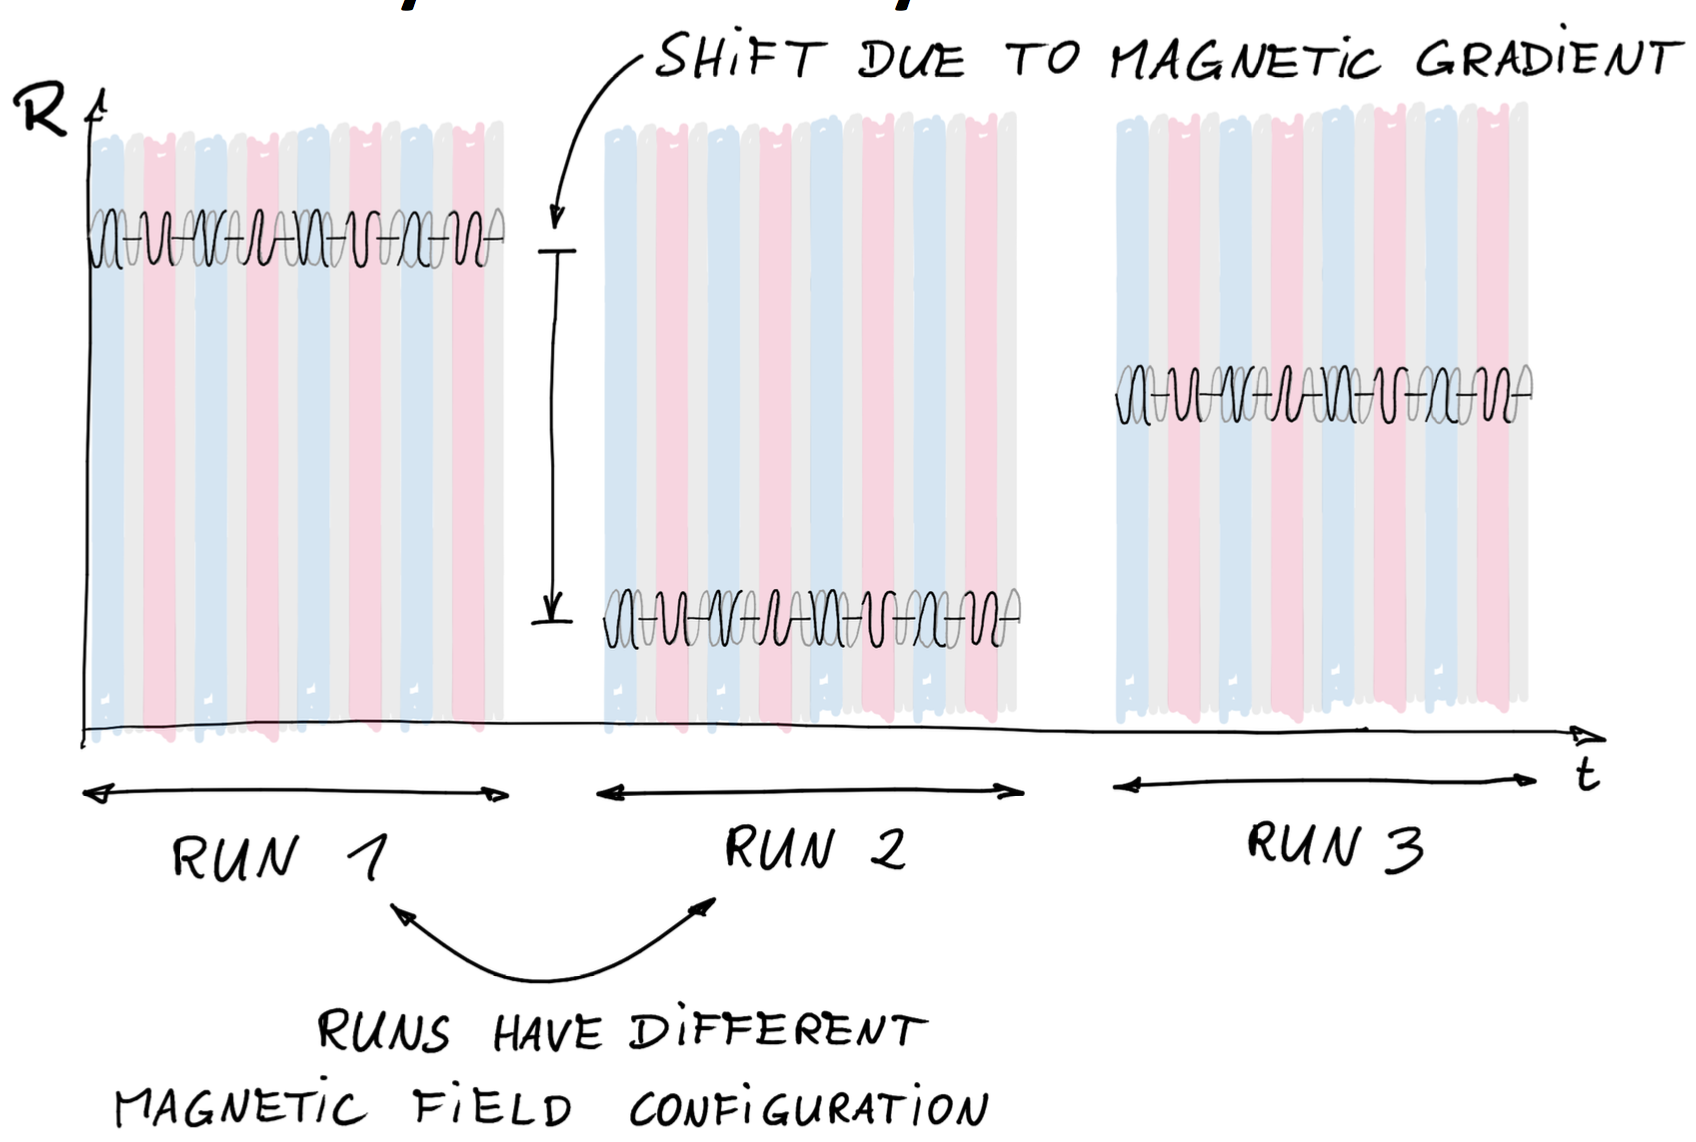
\includegraphics[width=.56\linewidth]{gfx/axions/cycle-level_gradient_jump.png}}
  \caption{The data taking scheme in the nEDM experiment at PSI.}
\end{figure}

A part of the measurement procedure is to deliberately work in a magnetic field gradient, as explained\ldots \mnote{Need to explain in somewhere, best at the beginning.} The vertical magnetic filed gradient changes substantially when a new run is started. \mnote{Give the reasons why it changes: we apply a new one, which follows from the measurement procedure} Thereby $R$ is shifted by a big value, changing the DC level of the oscillating nEDM signal, which is illustrated in Fig.\,\ref{fig:axions_data_taking_runs}. Moreover, even during a single run the gradient drifts, as clearly visible in Fig.\,\ref{fig:axions_gradient_drift_correction}. \mnote{Write here, that we can do a good relative gradient drift correction, but not an absolute one.}

\begin{figure}[bth]
  %FIXME directly copied from Elise's presentation on the 2015 PSI collaboration meeting
  \myfloatalign
  \subfloat
  [Another time series of $R$ in the nEDM experiment. The colours depict electric field states, black being no electric field. A drift is clearly visible.]
  {\label{fig:axions_gradient_drift_not_corrected}
  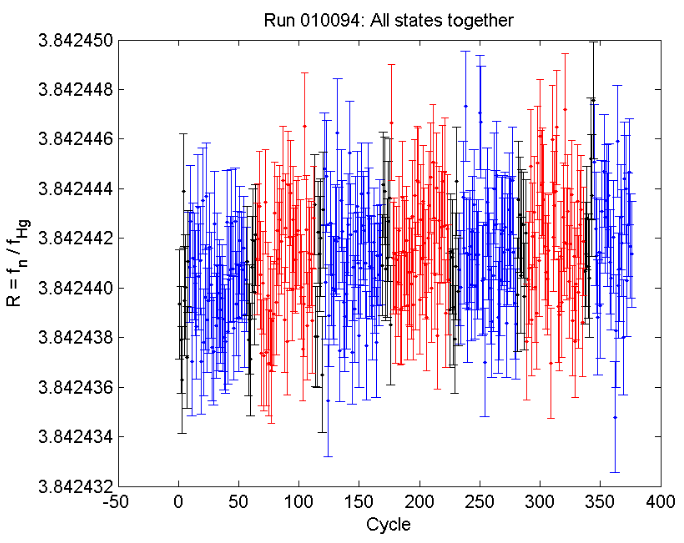
\includegraphics[width=.45\linewidth]{gfx/axions/gradient_drift_elise}}
  \quad
  \subfloat
  [The data as on Fig.\,\ref{fig:axions_gradient_drift_not_corrected} corrected for gradient fluctuations.]
  {\label{fig:axions_gradient_drift_corrected}
  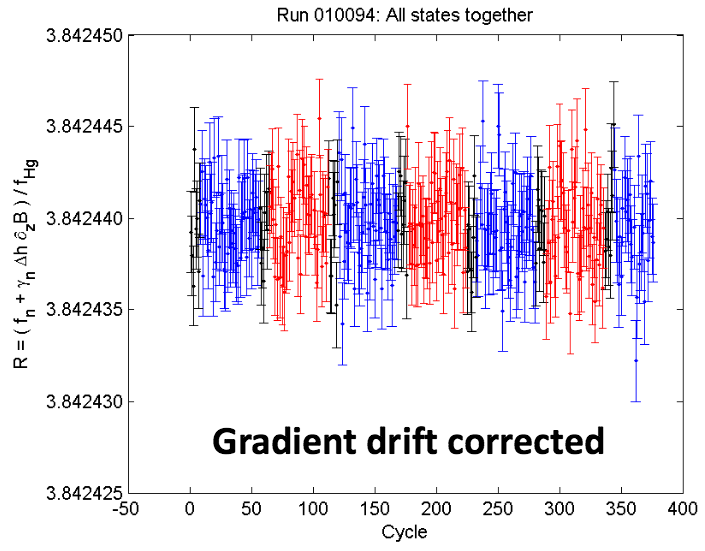
\includegraphics[width=.45\linewidth]{gfx/axions/gradient_drift_elise_corrected}}
  \caption{Correcting the $R$ time series for fluctuations of the vertical magnetic field gradient.}
  \label{fig:axions_gradient_drift_correction}
\end{figure}

The nEDM team spares no effort to measure the gradient. Nevertheless, the achieved precision ($\approx \unit[1]{pT/cm}$ is only comparable to the one of $f_n$ (in the order of \unit[1]{pT}). The exact way how the gradient should determined is highly non--trivial and there is ongoing research in this respect. \mnote{Mention here the exact way the gradient drift correction is done. And cite Elise's thesis.} Actually, even the height difference between the neturons and $^{199}$Hg centres of mass (a few milimeters) is still discussed. \mnote{Know how exactly was $\Delta h$ determined in the end. Also, mention the definition of a sequence here (as in the paper).} % Assuming a constant gradient during a \emph{run} one can determine it much more precise. This assumption, however, is known not to be exactly true.

One should note, that any, including an oscillating one, nEDM effect affects only the position of the neutrons' resonance. The shape of the resonance curve is unaffected. Therefore, the method to extract neutron Larmor frequency $f_n$, and thereby $R$, for each \emph{cycle} is valid also in case of an oscillating nEDM.

It may be tempting to think about demodulating the $R$ time--series into what would be expected to be an oscillation. This would require subtracting the DC offset for each electric field configuration, in each run separately, then flipping the signal around the DC level for one configuration. \mnote{The offsets are measured with Cs, mention that.} The disadvantage is that uncertainty in such a demodulation would become a systematic effect and would need to be tightly controlled.

A different approach, one that that was taken, is to split the $R$ time--series into three: without the electric field (a control data set, no signal expected), with the electric and magnetic field parallel, and with anti-parallel. Then in the LSSA fit instead of one DC offset, allow a different one for each run:

\begin{equation}
  A\sin(2 \pi f t) + B\cos(2 \pi f t) + \sum_i C_i\,\Pi_i(t) \, .
\end{equation}








\begin{figure}
  \centering 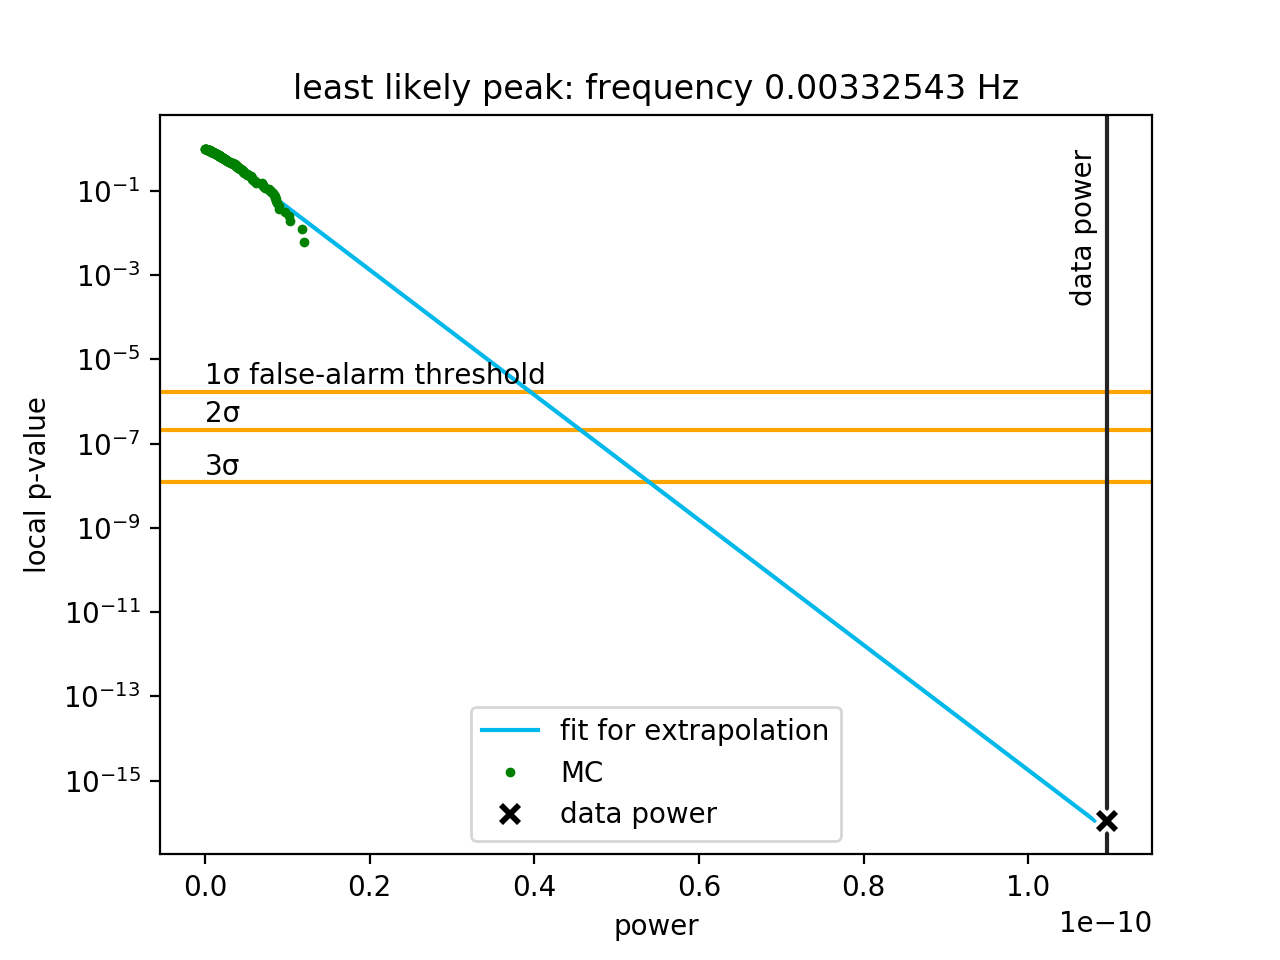
\includegraphics[width=\linewidth]{gfx/axions/P_best_signal_candidate.png}
  \caption{1 - CDF for the parallel dataset. This provides the power to local p-value trasition, for each frequency separately. The extrapolation based on Eq.\ldots is shown.}
  \label{fig:P_best_signal_candidate}
\end{figure}

\begin{figure}
  \centering 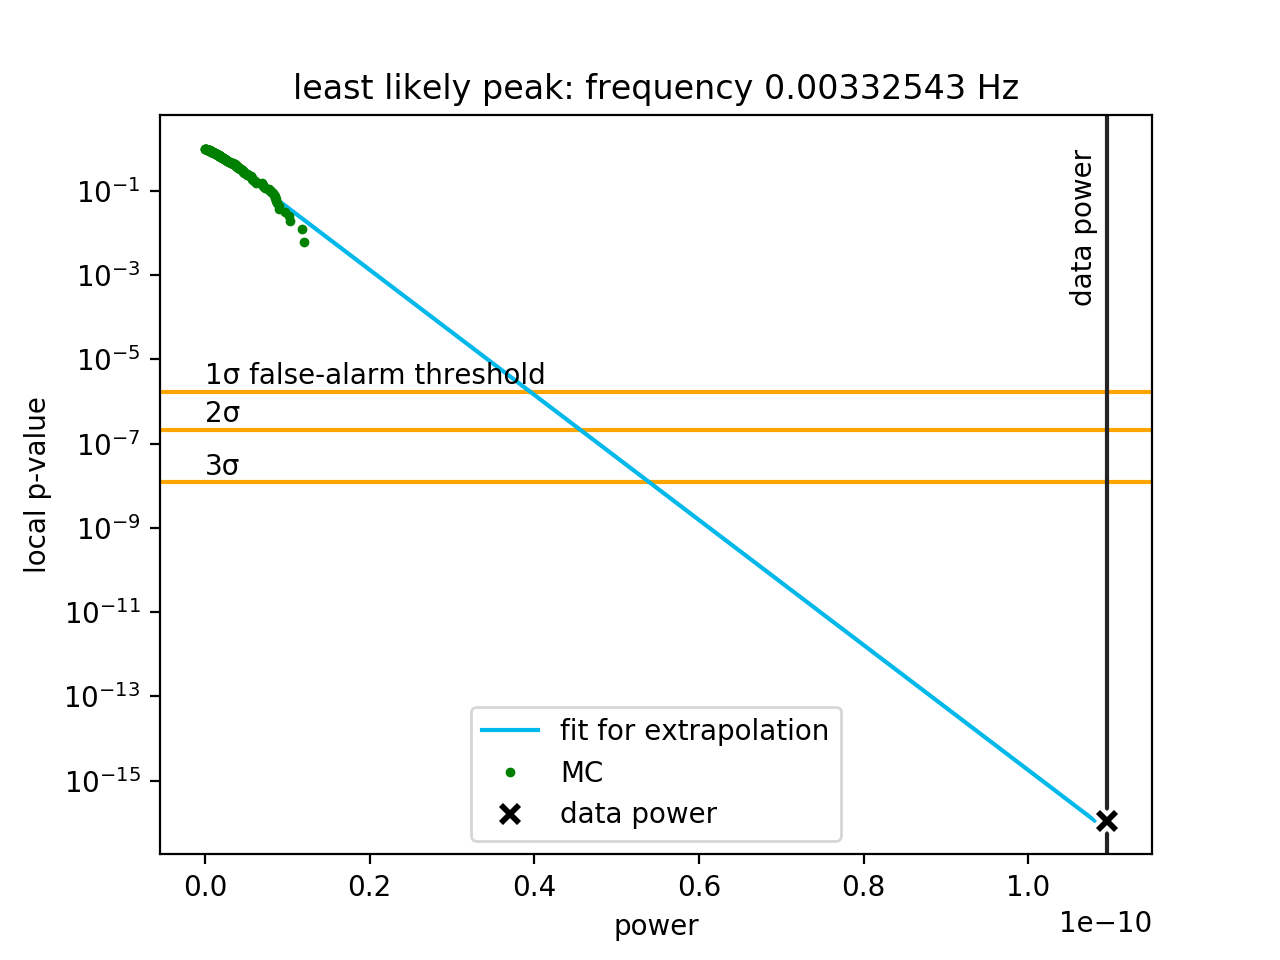
\includegraphics[width=\linewidth]{gfx/axions/P_best_signal_candidate.png}
  \caption{Accounting for the look-elsewhere effect for the parallel dataset. It provides the ''minimal local p-value`` -- global p-value transition. The fit with the model \dots gives the number of frequencies.}
  \label{fig:P_best_signal_candidate}
\end{figure}







\section{The analysis itself}

\section{Axion-Wind analysis}

\section{Comparison of the analyses}
